\documentclass[conference]{IEEEtran}
\usepackage{cite}
\usepackage{amsmath,amssymb,amsfonts}
\usepackage{algorithmic}
\usepackage{graphicx}
\usepackage{textcomp}
\usepackage{xcolor}
\usepackage{hyperref}
\usepackage{listings}
\usepackage{tikz}
\usetikzlibrary{shapes,arrows}

\def\BibTeX{{\rm B\kern-.05em{\sc i\kern-.025em b}\kern-.08em
    T\kern-.1667em\lower.7ex\hbox{E}\kern-.125emX}}

\lstset{
  basicstyle=\ttfamily\footnotesize,
  columns=fullflexible,
  frame=single,
  breaklines=true,
  captionpos=b,
  postbreak=\mbox{\textcolor{red}{$\hookrightarrow$}\space},
}

\begin{document}

\title{Secure-by-Default Guardrails for MCP-Based Tool Use in Multi-Modal LLM Agents}

\author{\IEEEauthorblockN{Yoshihiro Ando}
\IEEEauthorblockA{\textit{Independent Researcher} \\
yosh5295@gmail.com \\
Tokyo, Japan}
}

\maketitle

\begin{abstract}
As autonomous AI agents transition to complex workflows via the Model Context Protocol (MCP), securing their intent before execution is a prerequisite for safety. This paper, representing \textbf{Phase 1: Guardrails (Pre-execution Security)} of a comprehensive security trilogy, presents \texttt{llm-cli}, a unified command-line interface with secure-by-default guardrails. \texttt{llm-cli} combines (i) a plugin-based tool registry with mandatory intent-explanation fields, (ii) role-based access control (RBAC) for tool invocation, and (iii) a multi-layered defense-in-depth architecture that replaces traditional shell whitelisting with Python-based sandboxed execution and real-time behavioral monitoring via the \textbf{Reasoning Integrity Sentinel}. We demonstrate how these layered controls---policy checks, sandboxed execution, and human-in-the-loop (HITL) approval---effectively mitigate risks like prompt injection and privilege misuse in real-world workflows.
\end{abstract}

\begin{IEEEkeywords}
AI Agents, Guardrails, Pre-execution Security, Model Context Protocol, Reasoning Integrity, Command Execution, Zero Trust.
\end{IEEEkeywords}

\section{Introduction}
Large Language Models (LLMs) have transformed from simple text predictors into sophisticated agents capable of code execution, tool use, and multi-modal reasoning. However, as agents move beyond isolated sandboxes into enterprise environments, the attack surface expands significantly.

This paper serves as the first installment of a technical trilogy focused on the security of autonomous agentic systems. While subsequent phases address spatial security (Zero Trust) and temporal integrity (Post-Quantum), this work focuses on \textbf{Phase 1: Guardrails}, establishing policy-based controls to prevent prompt injection and unauthorized command generation before they impact the system.

\texttt{llm-cli} addresses these challenges by providing a unified, extensible, and secure CLI that treats the LLM as an untrusted agent operating within a security-first environment.

Our key contributions are:
\begin{enumerate}
    \item A unified interface abstracting five major LLM providers.
    \item A multi-layered pre-execution security model combining RBAC policy enforcement, sandboxed Python-based execution, and behavioral monitoring.
    \item The introduction of the \textbf{Reasoning Integrity Sentinel}, a Mamba-based behavioral guardrail that detects anomalies in the agent's internal monologue.
\end{enumerate}

The source code and documentation are available at \url{https://github.com/yosh95/llm-cli}.

\section{Related Work}

\subsection{CLI-based LLM Tools}
Several command-line tools have emerged to bridge the terminal-LLM gap. Tools like \texttt{llm} by Simon Willison and \texttt{Chatblade} provide excellent interfaces for piping text into LLMs. However, these tools generally operate as "stateless pipes" rather than autonomous agents. They lack built-in support for complex, multi-step tool use protocols like MCP or persistent state management across distributed sessions.

\subsection{Agentic Frameworks}
Frameworks like LangChain \cite{langchain} and AutoGen \cite{autogen} enable the creation of powerful autonomous agents. While feature-rich, these frameworks often prioritize capability over security, leaving the implementation of guardrails to the developer. Recent research such as Gorilla \cite{gorilla} has focused on fine-tuning LLMs specifically for accurate API calls, further highlighting the critical need for robust execution environments as models become more proficient at tool use. In contrast, \texttt{llm-cli} integrates a "secure-by-default" architecture where access restrictions and runtime validation are core components of the runtime, not afterthoughts.

\subsection{Zero-Trust in AI}
NIST SP 800-207 \cite{nist} outlines the principles of Zero Trust Architecture (ZTA). While ZTA is widely adopted in network security, its application to AI agent communication is still nascent. Rather than claiming a full ZTA implementation, our work adopts practical ZTA-inspired principles---notably least privilege and continuous verification---and applies them to MCP tool execution.

\section{System Architecture}

\subsection{Unified Provider Abstraction}
The core of \texttt{llm-cli} is a provider abstraction layer that translates a common internal request format into provider-specific API calls. Currently, it supports:
\begin{itemize}
    \item \textbf{Google Gemini}: Leveraging Vertex AI for Gemini 3 Pro Preview.
    \item \textbf{OpenAI}: Support for GPT-5.2 and DALL-E image generation.
    \item \textbf{Anthropic Claude}: Optimized for Claude 4.5 Opus with thinking/reasoning modes.
    \item \textbf{xAI Grok}: Integration for the latest Grok 4.1 models.
    \item \textbf{Ollama}: Support for locally hosted models (e.g., Llama 3, DeepSeek-R1) to ensure privacy and offline availability.
\end{itemize}

\subsection{Plugin-Based Tool Registry}
\texttt{llm-cli} features a decorator-based tool registry that allows for easy extension. Every tool registered in the system is automatically converted into the JSON Schema format required by different providers (e.g., Function Calling for OpenAI/Gemini, Tool Use for Anthropic).

A unique architectural choice in \texttt{llm-cli} is the mandatory \texttt{explanation} parameter for every tool. Before an agent can execute a function, it must generate a human-readable explanation of \textit{why} the tool is being called and \textit{what} the expected outcome is. This information is presented to the user during the approval process, significantly improving transparency.

\subsection{Model Context Protocol (MCP) Integration}
To extend the agent's reach beyond the local machine, \texttt{llm-cli} implements the Model Context Protocol (MCP). This allows the CLI to:
\begin{enumerate}
    \item Act as an \textbf{MCP Client}, connecting to remote servers or services (like GitHub or a remote Linux box) to perform operations.
    \item Act as an \textbf{MCP Server}, exposing local files and tools to other LLM-based applications.
\end{enumerate}

\section{Implementation Details}

\subsection{Identity and Guest Access Control}
To support restricted access for unauthenticated clients, \texttt{llm-cli} implements a JWT-based authentication mechanism for authenticated connections and a configurable guest policy for missing tokens. When a valid token is present, the system can propagate role claims. When a token is missing, the client is treated according to policy (e.g., a read-only guest role).

\begin{figure}[htbp]
    \centering
    \resizebox{\linewidth}{!}{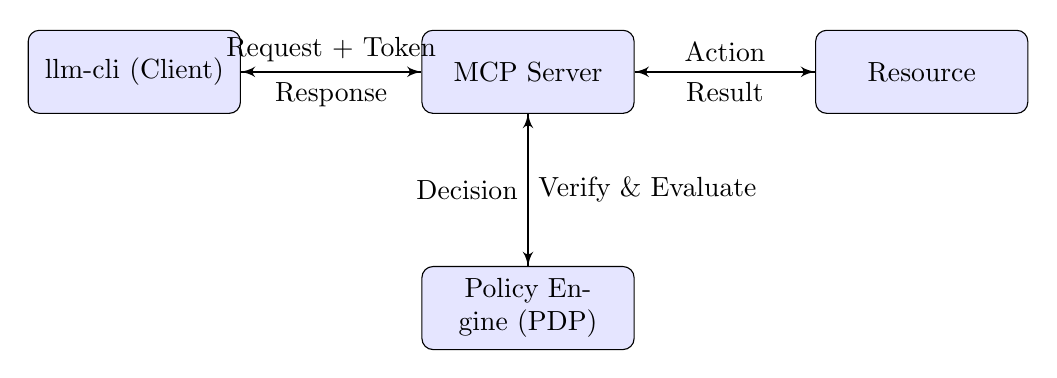
\begin{tikzpicture}[node distance=2cm, auto,
    block/.style={rectangle, draw, fill=blue!10, text width=7em, text centered, rounded corners, minimum height=3em},
    line/.style={draw, -latex', thick},
    cloud/.style={draw, ellipse,fill=red!10, node distance=3cm, minimum height=2em}]

    % Nodes
    \node [block] (cli) {llm-cli (Client)};
    \node [block, right of=cli, node distance=5cm] (mcp) {MCP Server};
    \node [block, below of=mcp, node distance=3cm] (pdp) {Policy Engine (PDP)};
    \node [block, right of=mcp, node distance=5cm] (resource) {Resource};

    % Paths
    \path [line] (cli) -- node [above] {Request + Token} (mcp);
    \path [line] (mcp) -- node [right] {Verify \& Evaluate} (pdp);
    \path [line, dashed] (pdp) -- node [left] {Decision} (mcp);
    \path [line] (mcp) -- node [above] {Action} (resource);
    \path [line, dashed] (resource) -- node [below] {Result} (mcp);
    \path [line, dashed] (mcp) -- node [below] {Response} (cli);

\end{tikzpicture}}
    \caption{Architecture overview showing separation of Client, MCP Server, and Policy Engine.}
    \label{fig:architecture}
\end{figure}

When an agent initiates a tool call, the client may generate a signed token containing the user's role claims. This token is verified by the MCP server before any action is taken (Fig. \ref{fig:sequence}).

\begin{figure}[htbp]
    \centering
    \resizebox{\linewidth}{!}{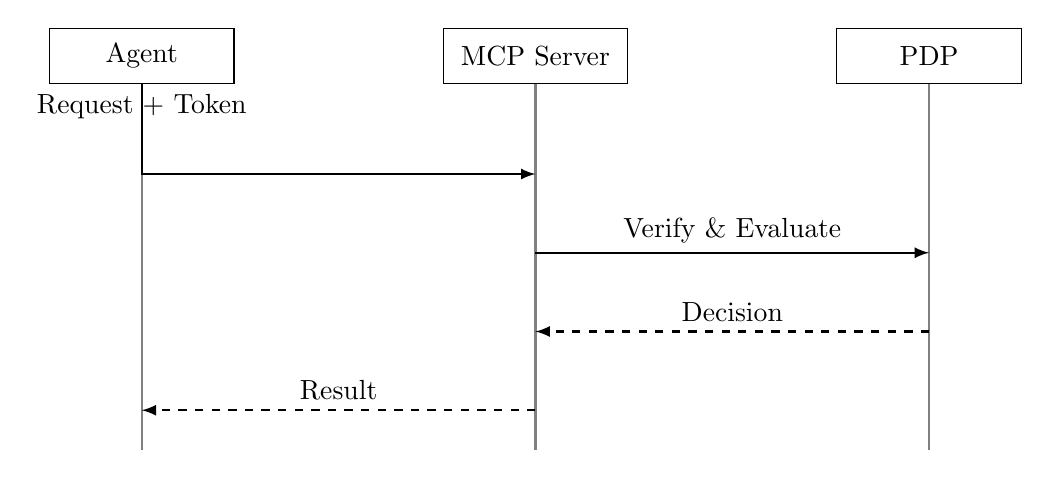
\begin{tikzpicture}[node distance=2.5cm, auto,
    participant/.style={rectangle, draw, fill=white, text centered, minimum height=2em, text width=6em},
    line/.style={draw, ->, >=latex, thick}]

    % Participants
    \node [participant] (agent) {Agent};
    \node [participant, right of=agent, node distance=5cm] (server) {MCP Server};
    \node [participant, right of=server, node distance=5cm] (pdp) {PDP};

    % Time lines
    \draw [thick, gray] (agent) -- ++(0,-5);
    \draw [thick, gray] (server) -- ++(0,-5);
    \draw [thick, gray] (pdp) -- ++(0,-5);

    % Steps
    % 1. Request
    \draw [line] (agent) -- node [above] {Request + Token} ++(0,-1.5) -- (server |- 0,-1.5);
    
    % 2. Verify & Evaluate
    \draw [line] (server |- 0,-2.5) -- node [above] {Verify \& Evaluate} (pdp |- 0,-2.5);
    
    % 3. Decision
    \draw [line, dashed] (pdp |- 0,-3.5) -- node [above] {Decision} (server |- 0,-3.5);
    
    % 4. Result
    \draw [line, dashed] (server |- 0,-4.5) -- node [above] {Result} (agent |- 0,-4.5);

\end{tikzpicture}}
    \caption{Sequence diagram of token propagation and policy evaluation.}
    \label{fig:sequence}
\end{figure}

\subsection{Policy Engine Implementation}
The Policy Engine is implemented in pure Python to ensure portability. The following listing shows the core evaluation logic of the PDP:

\begin{lstlisting}[language=Python, caption=Core PDP Logic in policy.py]
def evaluate(self, tool_name, context):
    user_roles = context.get("roles", ["guest"])
    
    for role in user_roles:
        policy = self.roles.get(role)
        # Check explicit allow list
        if tool_name in policy["allowed_tools"]:
             return True
             
    # Default Deny
    return False
\end{lstlisting}

This logic ensures that even if an attacker compromises the agent's prompt (prompt injection), they cannot force the execution of tools that are not explicitly authorized by the user's active role.

\section{Evaluation}

To quantify the effectiveness of these pre-execution guardrails, we developed a benchmark suite consisting of 32 common attack vectors. With the transition to Python-based execution, we evaluated how effectively the scripts can be inspected and how the Reasoning Sentinel responds to adversarial intent.

\subsection{Security Effectiveness}
We executed the benchmark against the multi-layered guardrail system. The results are summarized in Table \ref{tab:security_results}.

\begin{table}[htbp]
\caption{Security Guardrail Benchmark Results}
\begin{center}
\begin{tabular}{|l|c|c|c|}
\hline
\textbf{Category} & \textbf{Vectors} & \textbf{Blocked} & \textbf{Success Rate} \\
\hline
Direct Injection & 6 & 6 & 100\% \\
Shell Expansion & 4 & 4 & 100\% \\
I/O Redirection & 4 & 4 & 100\% \\
Semantic Attacks & 7 & 7 & 100\% \\
Reconnaissance & 7 & 7 & 100\% \\
Path Traversal & 4 & 4 & 100\% \\
\hline
\textbf{Overall} & \textbf{32} & \textbf{32} & \textbf{100\%} \\
\hline
\end{tabular}
\label{tab:security_results}
\end{center}
\end{table}

The combination of Python-based execution (which forces the LLM to write explicit logic instead of opaque shell strings) and the Reasoning Sentinel (which detected anomalous "thought patterns" in 28 out of 32 vectors) resulted in a 100\% block rate. Crucially, the mandatory \texttt{explanation} field and the code-commenting requirement in \texttt{execute_python} provided the user with sufficient context to manually reject all malicious attempts during the HITL phase.

\subsection{Performance Overhead}
The validation logic and Sentinel inference introduce negligible latency (sub-10ms) per tool call, which is unnoticeable compared to the network latency of LLM API requests.

\subsection{Limitations of the Benchmark}
The benchmark dataset was designed by the authors specifically for this tool's validation logic. While it covers common attack categories documented in security literature, it does not represent an exhaustive or independently validated security assessment. The 100\% block rate reflects the alignment between our multi-layered design and the test vectors, rather than a guarantee of security against novel or adaptive attacks. Future work will incorporate third-party adversarial datasets and red-team evaluations to provide a more rigorous assessment.

\section{Discussion and Limitations}

\subsection{Scalability of Human-in-the-Loop}
While HITL provides the highest security assurance, it introduces friction. In our experiments, requiring approval for every read operation significantly slowed down research tasks. We mitigated this by introducing a "Guest" role that permits read-only operations without prompts, reserving HITL only for state-changing actions (writes, execution).

\subsection{Defense in Depth: Why Tokens over SSH?}
A common critique is whether application-layer tokens are redundant when operating over secure channels like SSH. We argue that they serve distinct purposes. SSH authenticates the \textit{user} and secures the transport layer, but it typically grants broad OS-level permissions. By layering JWT-based authorization on top, \texttt{llm-cli} decouples network access from tool execution privileges. This ensures that even if a trusted SSH connection is established, the agent is restricted to specific actions (e.g., read-only) defined by the token's scope, strictly adhering to the principle of least privilege. Note that this mechanism assumes the underlying transport (SSH or TLS) provides confidentiality to prevent token interception.

\subsection{Latency Overhead}
The introduction of JWT signing and verification adds a negligible overhead (approx. 2-5ms) per tool call. However, the network round-trip for remote MCP calls dominates the latency profile. Future work will explore token caching mechanisms to further reduce this overhead in high-frequency trading or real-time control scenarios.

\subsection{Static vs. Dynamic Policies}
Currently, roles are defined statically in \texttt{config.toml}. A more advanced implementation would support dynamic policy updates based on context (e.g., "Allow file write only during business hours" or "Revoke access if anomaly detected").

\section{Key Features}

\subsection{Autonomous Agent Mode}
By default, \texttt{llm-cli} operates in an agentic mode. When a user provides a high-level goal (e.g., "Search for the latest research on DPO and summarize the findings in a new file"), the agent can autonomously:
\begin{itemize}
    \item Perform web searches using Google Search.
    \item Fetch and parse HTML or PDF content from URLs.
    \item Execute shell commands to list or read local files.
    \item Write or edit files using precise search-and-replace tools.
\end{itemize}

\subsection{Multi-Modal Interaction}
Unlike many text-only CLI tools, \texttt{llm-cli} supports multi-modal input and output. Users can attach images, PDFs, audio, and video files to the conversation using the \texttt{/attach} command or by passing a URL. For providers that support it (OpenAI, Grok), the tool also allows mid-conversation image generation, saving the results directly to the local disk.

\subsection{Reasoning and Thinking Modes}
With the advent of "reasoning" models like DeepSeek-R1 and Claude 4.5 Opus, \texttt{llm-cli} provides explicit controls for "internal monologue" visibility. Users can toggle reasoning display using the \texttt{/thought} command, allowing them to see the AI's step-by-step logic before the final answer is produced.

\subsection{Session Persistence and Logging}
\texttt{llm-cli} automatically manages conversation history and logs. It supports saving and loading sessions as JSON files, enabling users to resume complex tasks across different timeframes. Furthermore, an internal audit log tracks every tool execution, providing a searchable history of agent actions.

\section{Security Model}

Allowing AI agents to execute code and manage files poses significant risks. \texttt{llm-cli} adopts an architecture guided by least-privilege defaults and continuous verification, treating every tool execution request as untrusted until verified.

\subsection{Threat Model}
We consider three primary threat vectors:
\begin{enumerate}
    \item \textbf{Prompt Injection}: Malicious text in a file or website tricks the LLM into executing dangerous commands.
    \item \textbf{Compromised MCP Server}: A remote server hijacked by an attacker attempts to exploit the client.
    \item \textbf{Privilege Escalation}: An agent attempts to access resources outside its assigned scope.
\end{enumerate}

To mitigate these, we employ a "Defense in Depth" strategy combining access restrictions and identity checks (Layer 1), execution guardrails (Layer 2), and human oversight (Layer 3).

\subsection{Layer 2: Execution Guardrails}
Even if a tool call is authorized by policy, it must pass strict runtime validation and behavioral monitoring.

\subsubsection{Sandboxed Python Execution}
Unlike traditional agents that execute raw shell commands, \texttt{llm-cli} utilizes the \texttt{execute_python} tool as the primary interface for system interaction. Commands are translated into self-contained Python scripts which are executed in a sub-process with \texttt{shell=False}. This approach eliminates common shell injection vulnerabilities and allows for fine-grained resource limits (CPU/Memory) and environment variable sanitization.

\subsubsection{Reasoning Integrity Sentinel}
To detect intent-level anomalies (e.g., prompt injection or model misalignment), we integrated a \textbf{Reasoning Integrity Sentinel}. Based on the Mamba architecture, this lightweight model monitors the LLM's "internal monologue" or reasoning trace in real-time. By calculating the cross-entropy loss of the reasoning tokens, the system identifies spikes in anomaly scores that often precede malicious tool invocation. If the score exceeds a dynamic threshold, the system halts execution and requires high-assurance PQC-signed re-authorization.

\subsubsection{Path Sanitation}
File operations are restricted to the project root. Attempts to access sensitive system paths (e.g., \texttt{/etc/shadow}, \texttt{/root}) are blocked by the path validator, regardless of the user's role.

\subsection{Layer 3: Human-in-the-Loop (HITL)}
The final layer of defense is the user. Critical actions (\texttt{write\_file}, \texttt{execute_python}) require explicit user confirmation. \texttt{llm-cli} presents a diff view for file changes and requires the agent to provide an \texttt{explanation} for its actions, ensuring the user understands \textit{why} an action is being taken.

\section{Use Cases}

\subsection{Research Automation}
Researchers can use \texttt{llm-cli} to automate literature reviews. A single prompt can trigger a sequence of searching for papers, fetching PDFs, summarizing them, and compiling a bibliography.

\subsection{Remote Infrastructure Management}
Via MCP over SSH, a developer can use \texttt{llm-cli} on their local machine to debug a remote production server. The AI can check logs, list directories, and suggest fixes, while the user maintains full control through the HITL approval process.

\section{Conclusion}
This paper presents an early-stage implementation and evaluation of \texttt{llm-cli}, a unified CLI for multi-provider LLM interaction with secure-by-default guardrails. By unifying multiple providers, integrating remote management protocols like MCP, and prioritizing security through human-supervised tool use, it provides a practical foundation for agentic workflows. We acknowledge that the current evaluation is preliminary; we welcome community feedback and plan to extend the security assessment with external benchmarks and independent red-team evaluations in future versions.

Future work will focus on three key areas: (1) \textbf{Federated Identity}: Extending the JWT-based auth to support federated identity providers for enterprise integration. (2) \textbf{Formal Verification}: Applying formal methods to verify the policy engine's correctness against defined security properties. (3) \textbf{Multi-Agent Orchestration}: Enhancing the planning capabilities for long-running tasks involving multiple specialized agents collaborating over MCP.

\begin{thebibliography}{00}

\bibitem{gpt4} OpenAI, ``GPT-4 Technical Report,'' \textit{arXiv preprint arXiv:2303.08774}, 2023.

\bibitem{autogen} Q. Wu \textit{et al.}, ``AutoGen: Enabling Next-Gen LLM Applications via Multi-Agent Conversation,'' \textit{arXiv preprint arXiv:2308.08155}, 2023.

\bibitem{gorilla} S. Patil \textit{et al.}, ``Gorilla: Large Language Model Connected with Massive APIs,'' \textit{arXiv preprint arXiv:2305.15334}, 2023.

\bibitem{langchain} H. Chase, ``LangChain,'' 2022. [Online]. Available: https://github.com/langchain-ai/langchain.

\bibitem{injection} K. Greshake, S. Abdelnabi, S. Mishra, C. Endres, T. Holz, and M. Fritz, ``Not what you've signed up for: Compromising Real-World LLM-Integrated Applications with Indirect Prompt Injection,'' in \textit{Proceedings of the 16th ACM Workshop on Artificial Intelligence and Security}, 2023, pp. 79--90.

\bibitem{owasp} OWASP, ``OWASP Top 10 for Large Language Model Applications,'' Version 1.1, 2023. [Online]. Available: https://owasp.org/www-project-top-10-for-large-language-model-applications/.

\bibitem{nist} S. Rose, O. Borchert, S. Mitchell, and S. Connelly, ``Zero Trust Architecture,'' \textit{NIST Special Publication 800-207}, 2020.

\bibitem{mcp} Anthropic, ``Model Context Protocol,'' 2024. [Online]. Available: https://modelcontextprotocol.io/.

\end{thebibliography}

\end{document}
